% Chapter Template

\chapter{Implementation} % Main chapter title

\label{Chapter4} % Change X to a consecutive number; for referencing this chapter elsewhere, use \ref{ChapterX}

\lhead{Chapter X. \emph{Chapter Title Here}} % Change X to a consecutive number; this is for the header on each page - perhaps a shortened title

%----------------------------------------------------------------------------------------
%	SECTION 1
%----------------------------------------------------------------------------------------

\section{Introduction}

In order to perform the experiment it was necessary to implement the defeasible reasoning software as designed in the previous chapter.  
%   \begin{figure}[h!]
% \begin{center}
% \begin{tikzpicture}[->,>=stealth',shorten >=1pt,auto,node distance=2.5cm, semithick, scale=0.95, ,transform shape, align=left] 
% \tikzstyle{every state}=[fill=white,draw=black,text=black, font=\tiny, minimum size=5mm] 
%  \tikzstyle{EdgeStyle}=[bend left, font=\tiny] 
 
%  %central
% \node[state] at(-8,1) (SD1) {SD1}; 
% \node[state] at(-7,0) (SD2) {SD2};
% \node[state] at(-6,0) (SD3) {SD3};
% \node[state] at(-5,1) (SD4) {SD4};

% %mental demand
% \node[state] at(-8,2) (MD1) {MD1};
% \node[state] at(-7,3) (MD2) {MD2};
% \node[state] at(-6,3) (MD3) {MD3};
% \node[state] at(-5,2) (MD4) {MD4};

% %context bias
% \node[state] at(-8,4.5) (CB1) {CB1};
% \node[state] at(-7,4) (CB2) {CB2};
% \node[state] at(-6,4) (CB3) {CB3};
% \node[state] at(-5,4.5) (CB4) {CB4};

% %stress
% \node[state] at(-7,5.5) (PS1) {PS1};
% \node[state] at(-6,5.5) (PS2) {PS2};

% %effort
% \node[state] at(-8,8) (EF1) {EF1};
% \node[state] at(-7,8) (EF2) {EF2};
% \node[state] at(-6,8) (EF3) {EF3};
% \node[state] at(-5,8) (EF4) {EF4};

% %
% \node[state] at(-4,7) (DS1) [double] {DS1};


% %motivation mitigating
% \node[state] at(-8,6.5) (MV3) [double] {MV3};
% \node[state] at(-7,6.5) (MV5) [double] {MV5};
% \node[state] at(-5,6.5) (MV2) [double] {MV2};
% \node[state] at(-6,6.5) (MV4) [double] {MV4};


% %motivation forecast
% \node[state] at(-6,9.5) (MV1) {MV1};


% %past knowledge
% \node[state] at(-7,9.5) (PK1) {PK1};
% \node[state] at(-5.5,11.5) (PK2) {PK2};

% %skills
% \node[state] at(-8,10) (SK1) {SK1};
% \node[state] at(-7.0,11.5) (SK2) {SK2};

% \node[state] at(4,11.5) (SR1) {SR1};
% \node[state] at(3,11.5) (SR2) {SR2};
% \node[state] at(2,11.5) (SR3) {SR3};
% \node[state] at(1,11.5) (SR4) {SR4};

% \node[state] at(-1,11.5) (TS1) {TS1};
% \node[state] at(-2,11.5) (TS2) {TS2};
% \node[state] at(-3,11.5) (TS3) {TS3};
% \node[state] at(-4,11.5) (TS4) {TS4};

% \node[state] at(3.8,0) (VM1) {VM1};
% \node[state] at(2.8,0) (VM2) {VM2};
% \node[state] at(1.8,0) (VM3) {VM3};
% \node[state] at(0.8,0) (VM4) {VM4};

% \node[state] at(-1,0) (VR1) {VR1};
% \node[state] at(-2,0) (VR2) {VR2};
% \node[state] at(-3,0) (VR3) {VR3};
% \node[state] at(-4,0) (VR4) {VR4};

% \node[state] at(-3.8,2.5) (AR1) {AR1};
% \node[state] at(-2.8,2.5) (AR2) {AR2};
% \node[state] at(-1.8,2.5) (AR3) {AR3};
% \node[state] at(-0.8,2.5) (AR4) {AR4};

% \node[state] at(4,1.5) (MR1) {MR1};
% \node[state] at(3,1.5) (MR2) {MR2};
% \node[state] at(2,1.5) (MR3) {MR3};
% \node[state] at(1,1.5) (MR4) {MR4};

% %
% \node[state] at(-0.5,1.3) (SP1) {SP1};
% \node[state] at(-1.5,1.3) (SP2) {SP2};
% \node[state] at(-2.5,1.3) (SP3) {SP3};
% \node[state] at(-3.5,1.3) (SP4) {SP4};


% %
% \node[state] at(-3.5,10.5) (TD1) {TD1};
% \node[state] at(-2.5,10.5) (TD2) {TD2};
% \node[state] at(-1.5,10.5) (TD3) {TD3};
% \node[state] at(-0.5,10.5) (TD4) {TD4};

% %
% \node[state] at(-2,6) (PF1) {PF1};
% \node[state] at(-2,9.3) (PF2) {PF2};
% \node[state] at(2,10) (PF3) {PF3};
% \node[state] at(2,6) (PF4) {PF4};

% %
% \node[state] at(3.8,2.8) (PA1) {PA1};
% \node[state] at(2.8,2.8) (PA2) {PA2};
% \node[state] at(1.8,2.8) (PA3) {PA3};
% \node[state] at(0.8,2.8) (PA4) {PA4};

% \node[state] at(4,6) (AD1a) [double] {AD1a};
% \node[state] at(4,5) (AD2a) [double] {AD2a};
% \node[state] at(3.0,4) (AD6c) [double] {AD6c};
% \node[state] at(1,4) (AD5c) [double] {AD5c};
% \node[state] at(0.5,6.3) (AD3b) [double] {AD3b};
% \node[state] at(3.5,7) (AD4f) [double] {AD4f};
% \node[state] at(1.2,7.5) (AD4c) [double] {AD4c};



% \node[state] at(-4.2,5.5) (AD3a) [double] {AD3a};
% \node[state] at(-3.6,4) (AD4a) [double] {AD4a};
% \node[state] at(-1.8,4) (AD5a) [double] {AD5a};
% \node[state] at(-0.3,4) (AD5d) [double] {AD5d};
% \node[state] at(-0.1,5) (AD4d) [double] {AD4d};

% \node[state] at(-3,7) (DS2) [double] {DS2};
% \node[state] at(-1,7) (DS3) [double] {DS3};
% \node[state] at(-0.5,6) (DS4) [double] {DS4};


% \node[state] at(4,9) (AD5f) [double] {AD5f};
% \node[state] at(4,10.5) (AD4e) [double] {AD4e};
% \node[state] at(1,10.5) (AD6b) [double] {AD6b};
% \node[state] at(1,9) (AD1b) [double] {AD1b};



% \node[state] at(-3.5,8) (AD5b) [double] {AD5b};
% \node[state] at(-2,8) (AD5e) [double] {AD5e};
% \node[state] at(2.3,8) (AD2b) [double] {AD2b};
% \node[state] at(3.5,8) (AD4b) [double] {AD4b};
% \node[state] at(-4,9) (AD6a) [double] {AD6a};
% \node[state] at(-0,9) (AD1c) [double] {AD1c};
% \node[state] at(0,7.5) (AD2c) [double] {AD2c};

% %\path
% %(MV3) [bend left, ->,  dashed] edge  node {uc3} (EF1)
% %(MV5) [bend left, ->,  dashed] edge node {uc4}  (EF2)
% %(MV4) [bend left, ->,  dashed] edge node {uc1}  (EF3)
% %(MV2) [bend left, ->,  dashed] edge node {uc2} (EF4)
% %(AD3a) [bend left, ->,  dashed] edge node {um7} (PF1)
% %(AD4a) [bend left, ->,  dashed] edge node {um9} (PF1)
% %(AD5a) [bend left, ->,  dashed] edge node {um15} (PF1)
% %(AD4d) [bend left, ->,  dashed] edge node {um12} (PF1)
% %(AD5d) [bend left, ->,  dashed] edge node {um18} (PF1)
% %(AD1c) [bend left, ->,  dashed] edge node {um3} (PF2)
% %(AD2c) [bend left, ->,  dashed] edge node {um6} (PF2)
% %(AD5b) [bend left, ->,  dashed] edge node {um16} (PF2)
% %(AD5e) [bend left, ->,  dashed] edge node {um19} (PF2)
% %(AD6a) [bend left, ->,  dashed] edge node {um21} (PF2)
% %(AD1b) [bend left, ->,  dashed] edge node {um2} (PF3)
% %(AD2b) [bend left, ->,  dashed] edge node {um4} (PF3)
% %(AD4b) [bend left, ->,  dashed] edge node {um10} (PF3)
% %(AD5f) [bend left, ->,  dashed] edge node {um20} (PF3)
% %(AD6b) [bend left, ->,  dashed] edge node {um22} (PF3)
% %(AD5c) [bend left, ->,  dashed] edge node {um17} (PF4)
% %(AD4e) [bend left, ->,  dashed] edge node {um13} (PF3)
% %(AD1a) [bend left, ->,  dashed] edge node {um1} (PF4)
% %(AD2a) [bend left, ->,  dashed] edge node {um4} (PF4)
% %(AD3b) [bend left, ->,  dashed] edge node {um8} (PF4)
% %(AD4c) [bend left, ->,  dashed] edge node {um11} (PF4)
% %(AD4f) [bend left, ->,  dashed] edge node {um14} (PF4)
% %(AD6c) [bend left, ->,  dashed] edge node {um23} (PF4)
% %(DS2) [bend left, ->,  dashed] edge node {uc6} (PF1)
% %(DS3) [bend left, ->,  dashed] edge node {uc7} (PF1)
% %(DS4) [bend left, ->,  dashed] edge node {uc8} (PF1)
% %(DS1) [bend left, ->,  dashed] edge node {uc5} (EF4)
% %(MD1) [bend left, <->, solid] edge node {r1} (SD4)
% %(MD4) [bend left, <->] edge node {r2} (SD1)
% %(PK1) [bend left, <->] edge node {r3} (SK2)
% %(PK2) [bend left, <->] edge node {r4} (SK1)
% %(PK1) [bend right, <->] edge node {r5} (EF1)
% %(PK2) [bend left, <->] edge node {r6} (EF4)
% %(SK1) [bend right, <->] edge node {r7} (EF1)
% %(SK2) [bend left, <->] edge node {r8} (EF4)
% %(CB4) [bend left, <->] edge node {r9} (PS1)
% %; 

% \path
% (MV3) [bend left, ->,  dashed] edge  node {} (EF1)
% (MV5) [bend left, ->,  dashed] edge node {}  (EF2)
% (MV4) [bend left, ->,  dashed] edge node {}  (EF3)
% (MV2) [bend left, ->,  dashed] edge node {} (EF4)
% (AD3a) [bend left, ->,  dashed] edge node {} (PF1)
% (AD4a) [bend left, ->,  dashed] edge node {} (PF1)
% (AD5a) [bend left, ->,  dashed] edge node {} (PF1)
% (AD4d) [bend left, ->,  dashed] edge node {} (PF1)
% (AD5d) [bend left, ->,  dashed] edge node {} (PF1)
% (AD1c) [bend left, ->,  dashed] edge node {} (PF2)
% (AD2c) [bend left, ->,  dashed] edge node {} (PF2)
% (AD5b) [bend left, ->,  dashed] edge node {} (PF2)
% (AD5e) [bend left, ->,  dashed] edge node {} (PF2)
% (AD6a) [bend left, ->,  dashed] edge node {} (PF2)
% (AD1b) [bend left, ->,  dashed] edge node {} (PF3)
% (AD2b) [bend left, ->,  dashed] edge node {} (PF3)
% (AD4b) [bend left, ->,  dashed] edge node {} (PF3)
% (AD5f) [bend left, ->,  dashed] edge node {} (PF3)
% (AD6b) [bend left, ->,  dashed] edge node {} (PF3)
% (AD5c) [bend left, ->,  dashed] edge node {} (PF4)
% (AD4e) [bend left, ->,  dashed] edge node {} (PF3)
% (AD1a) [bend left, ->,  dashed] edge node {} (PF4)
% (AD2a) [bend left, ->,  dashed] edge node {} (PF4)
% (AD3b) [bend left, ->,  dashed] edge node {} (PF4)
% (AD4c) [bend left, ->,  dashed] edge node {} (PF4)
% (AD4f) [bend left, ->,  dashed] edge node {} (PF4)
% (AD6c) [bend left, ->,  dashed] edge node {} (PF4)
% (DS2) [bend left, ->,  dashed] edge node {} (PF1)
% (DS3) [bend left, ->,  dashed] edge node {} (PF1)
% (DS4) [bend left, ->,  dashed] edge node {} (PF1)
% (DS1) [bend left, ->,  dashed] edge node {} (EF4)
% ;

% \path
% (MD1) [bend left, <->, solid] edge node {} (SD4)
% (MD4) [bend left, <->] edge node {} (SD1)
% (PK1) [bend left, <->] edge node {} (SK2)
% (PK2) [bend left, <->] edge node {} (SK1)
% (PK1) [bend right, <->] edge node {} (EF1)
% (PK2) [bend left, <->] edge node {} (EF4)
% (SK1) [bend right, <->] edge node {} (EF1)
% (SK2) [bend left, <->] edge node {} (EF4)
% (CB4) [bend left, <->] edge node {} (PS1)
% ; 

% \end{tikzpicture} 
 
% \caption{The brand new instance: Knowledge-base translated into an argumentation graph}
% \label{fig:knowledgebaseargframework}
% \end{center}
% \end{figure}

%-----------------------------------
%	SUBSECTION 1
%-----------------------------------
\subsection{Subsection 1}



%-----------------------------------
%	SUBSECTION 2
%-----------------------------------

\subsection{Subsection 2}

%----------------------------------------------------------------------------------------
%	SOFTWARE IMPLEMENTATION
%----------------------------------------------------------------------------------------

\section{Software Implementation}

It was decided that the software would be implemented as a web application. This meant that the software could be accessed remotely from a number of different devices and would allow the expert to develop their knowledge base without having the software installed on their local machine. It also meant that the experimenter had access to the experts knowledge bases that had been saved to the system.

%-----------------------------------
%	SYSTEM ARCHITECTURE
%-----------------------------------
\subsection{System Architecture}

The implementation of the application uses a Javascript based front end with a RESTful Web Service based back-end written in PHP (using the Slim framework) and Java. 

The RESTful Web Service back-end provides a number of basic functions for the application. The back-end saves a knowledge base to disk as a JSON file and can similarly retrieve a list of knowledge bases and an individual knowledge base for the user. Knowledge bases were saved as JSON on disk rather than in a database as it eased the development process and would allow a knowledge base to be examined in it's complete form without needing assemble it with queries from the database. The back-end also allows the expert to load a small number of rows from the experiment data-set in order to evaluate the correctness of their knowledge-base.

The most important function of the back-end is to take a row from the data set and compute the value of the construct using the knowledge-base. The details of how this occurs are outlined later in this chapter.

%-----------------------------------
%	SYSTEM ARCHITECTURE
%-----------------------------------
\subsection{Application Front End}

A number of frameworks and libraries have been utilised in the development of the front-end. Bootstrap and JQuery have been used for presentational aspects of the site. Bootstrap provides a number of different useful components such as modal boxes allow the software to present information to the user in a clear manner. JQuery provides functionality such as DOM manipulation and AJAX networking facilities. 
A crucial component of the software is the development of argumentation frameworks and membership functions. This is achieved using the D3 library developed by Bostock et al.\cite{2011-d3} D3.js is a data visualisation library that allows developers and designer to load data and interact with the DOM using the data. Two key functionalities of D3 that are used in the implementation of the software are it's implementation of Bezier curves and it's force directed graph implementation.

Force directed graphs attempt to solve the problems posed when visualising graph data structures. Typical data visualisation techniques take values and parse them one by one, drawing some value in a position, drawing the next value next to it and so forth. This is not the case in graph data structures as generally it is prefered to have vertices that have common edges close together and to have those without common edges far apart. D3 provides a solution to this problem in the form of it's force directed techniques. The techniques take list of vertices and edges and generate positions for vertices using simulation inspired by physics. Similarly to sub-atomic particles, nodes are given a charge that repel other nodes in the graph. Nodes are from drifting apart by the links in the graph. There is also a force at the center of the visualisation that any of the nodes from drifting outside the viewport. 

The algorithms for generating the positions of the nodes are implemented in the D3 `force' layout. By utilising this layout and D3's event helpers (listeners for mouse actions such as click and drag) an interface can be implemented that allows a user to input a directed graph. This is the implementation that allows an expert to input an abstract argumentation framework.

By selecting a node in the graph representing an argument a user can then define membership functions representing premises and an output function. They do this by manipulating control points on a Bezier curve. D3 allows us to draw these curves and control points using SVG, which defines it's `paths' (Bezier curves) using control points. The membership functions and output function are defined simply as control points in the data model. The server uses algorithms to compute an output given an input value and a set of control points. In order to make these algorithms accessible to the reader a brief explanation of Bezier curves follows.

%-----------------------------------
%	BEZIER CURVES
%-----------------------------------

\subsection{Bezier Curves}

A Bezier Curve is a curve produced by a parameterised equation that produces a 

\subsection{Backend Implementation}

The basic functions of the backend such as storage and retrieval of data have been explained in section 1 of this chapter. The most crucial function of the back end is to take a row in the dataset and determine what a value for the construct associated with that row based on the knowledge base. In order to do this the javascript client makes a HTTP Post request to the base URL of the backend. This post request contains a JSON object which includes the expert's knowledge base, the row in the dataset and a list of semantics that are to be computed.

Once this request is parsed by the backend, irrelevant arguments and their associated links are removed from the graph. This is achieved by looking at an arguments membership functions. If the row in the dataset doesn't have a value between the minimum and maximum value of all premises in the argument then this argument is not activated and can be removed.

\begin{algorithm}
\caption{Determine activated arguments}
\begin{algorithmic} 
\FOR{each argument $arg$ \Pisymbol $N$ }
    % \FOR{each membership function $prem$ \Pisymbol{psy}{206} $arg$}
    %     $Val$ \leftarrow the column in the data corresponding to the premise
    %     \IF{$Val$ < $prem$\rightarrow$min$ OR $Val$ > $prem$\rightarrow$max$}
    %         Remove($arg$)
    %     \ENDIF
    % \ENDFOR
\ENDFOR
\end{algorithmic}
\end{algorithm}

The sub-graph of activated arguments and their relationships produced by this step is then formatted and passed into a Java program that computes the semantics. The main functionality of this code is known as the Dung-o-matic and is released under the Apache License, Version 2.0. The Dung-o-matic is an efficient implementation of a Dung argumentation framework that is used in this project to compute the semantics of the graph. The Dung-o-matic is wrapped in a main function that takes three command line arguments: an array of nodes, and array of links between nodes and a list of semantics to be computed. This program has been exported as a JAR file which is then called from PHP using the \lstinline{exec()} function. The Java code returns JSON object with the semantic names as keys and the sub-graphs as an array of arrays associated with those keys.

Once the semantics have been computed for an Argumentation Framework the values associated with each argument can be computed. For a given row in the data set, the results for an argument remain the same no mater what the configuration of the framework is. This allows us to cache the output value of an argument in memory rather than having to recompute the same values for each semantic. The results are computed on the server using a bBzier curve implementation.

If the output function of an argument is labeled as a mitigating argument then that argument is ignored.

%scaling of bezier curves

For a given membership function with fixed values for it's control points any point on the curve can be described by a value t between 0 and 1. By passing t into the function we obtain a value for x and y. As it is not possible to simply pass in an x value and obtain a corresponding y value we must search for y by varying the parameter t. This is done efficiently using a binary search algorithm. For each iteration we pass in two values of t to get two values of x and compare them with our target x value. We continue to search a space closer and smaller to x until we arrive at a value that is within a threshold we consider to be satisfactory. The value of t at this point gives the y value.

This calculation is performed for each membership function in the node and an average of the values of the output is produced. This corresponds to the overall degree of truth for the argument. This value is then used as the input to the output function which computes an overall construct value for that argument. 

Once the all of the construct values and degrees of truth are taken the averages of both values are taken. These are considered to be the Degree of Truth of that semantic and the construct value for that semantic. This is returned along with a list of the arguments for that semantic to the client. The client presents this to the user so that the user can evaluate whether or not their knowledge base is behaving in a manner that they expect it to or not.

% Semantic algorithms

%-----------------------------------
%	EXPERIMENT IMPLEMENTATION
%-----------------------------------
\section{Experiment Implementation}

The software implemented as above was used by both an expert in mental work load and a lay person. Both were asked to describe their knowledge of mental workload as a defeasible knowledge base and the knowledge bases were collected on the server.

As computing the semantics for an AF is an NP complete problem it is not yet possible to compute the results for a whole data set in the time that it would take to complete a typical HTTP request-response cycle. For the purposes of the experiment the functionality to compute the results for a whole data set using a given knowledge base was wrapped in a command line tool written in PHP. In order to reduce the time taken to compute the results and so as to focus the analysis of the experiment only the grounded and preferred extensions were computed. These overall degree of truth for the semantic and the value of MWL for the row in the dataset were stored for later analysis.

%-----------------------------------
%	SUBSECTION 1
%-----------------------------------
\subsection{Weka}



%-----------------------------------
%	SUBSECTION 2
%-----------------------------------

\subsection{Knowledge Base Elicitation}

\begin{figure}[H]
\centering
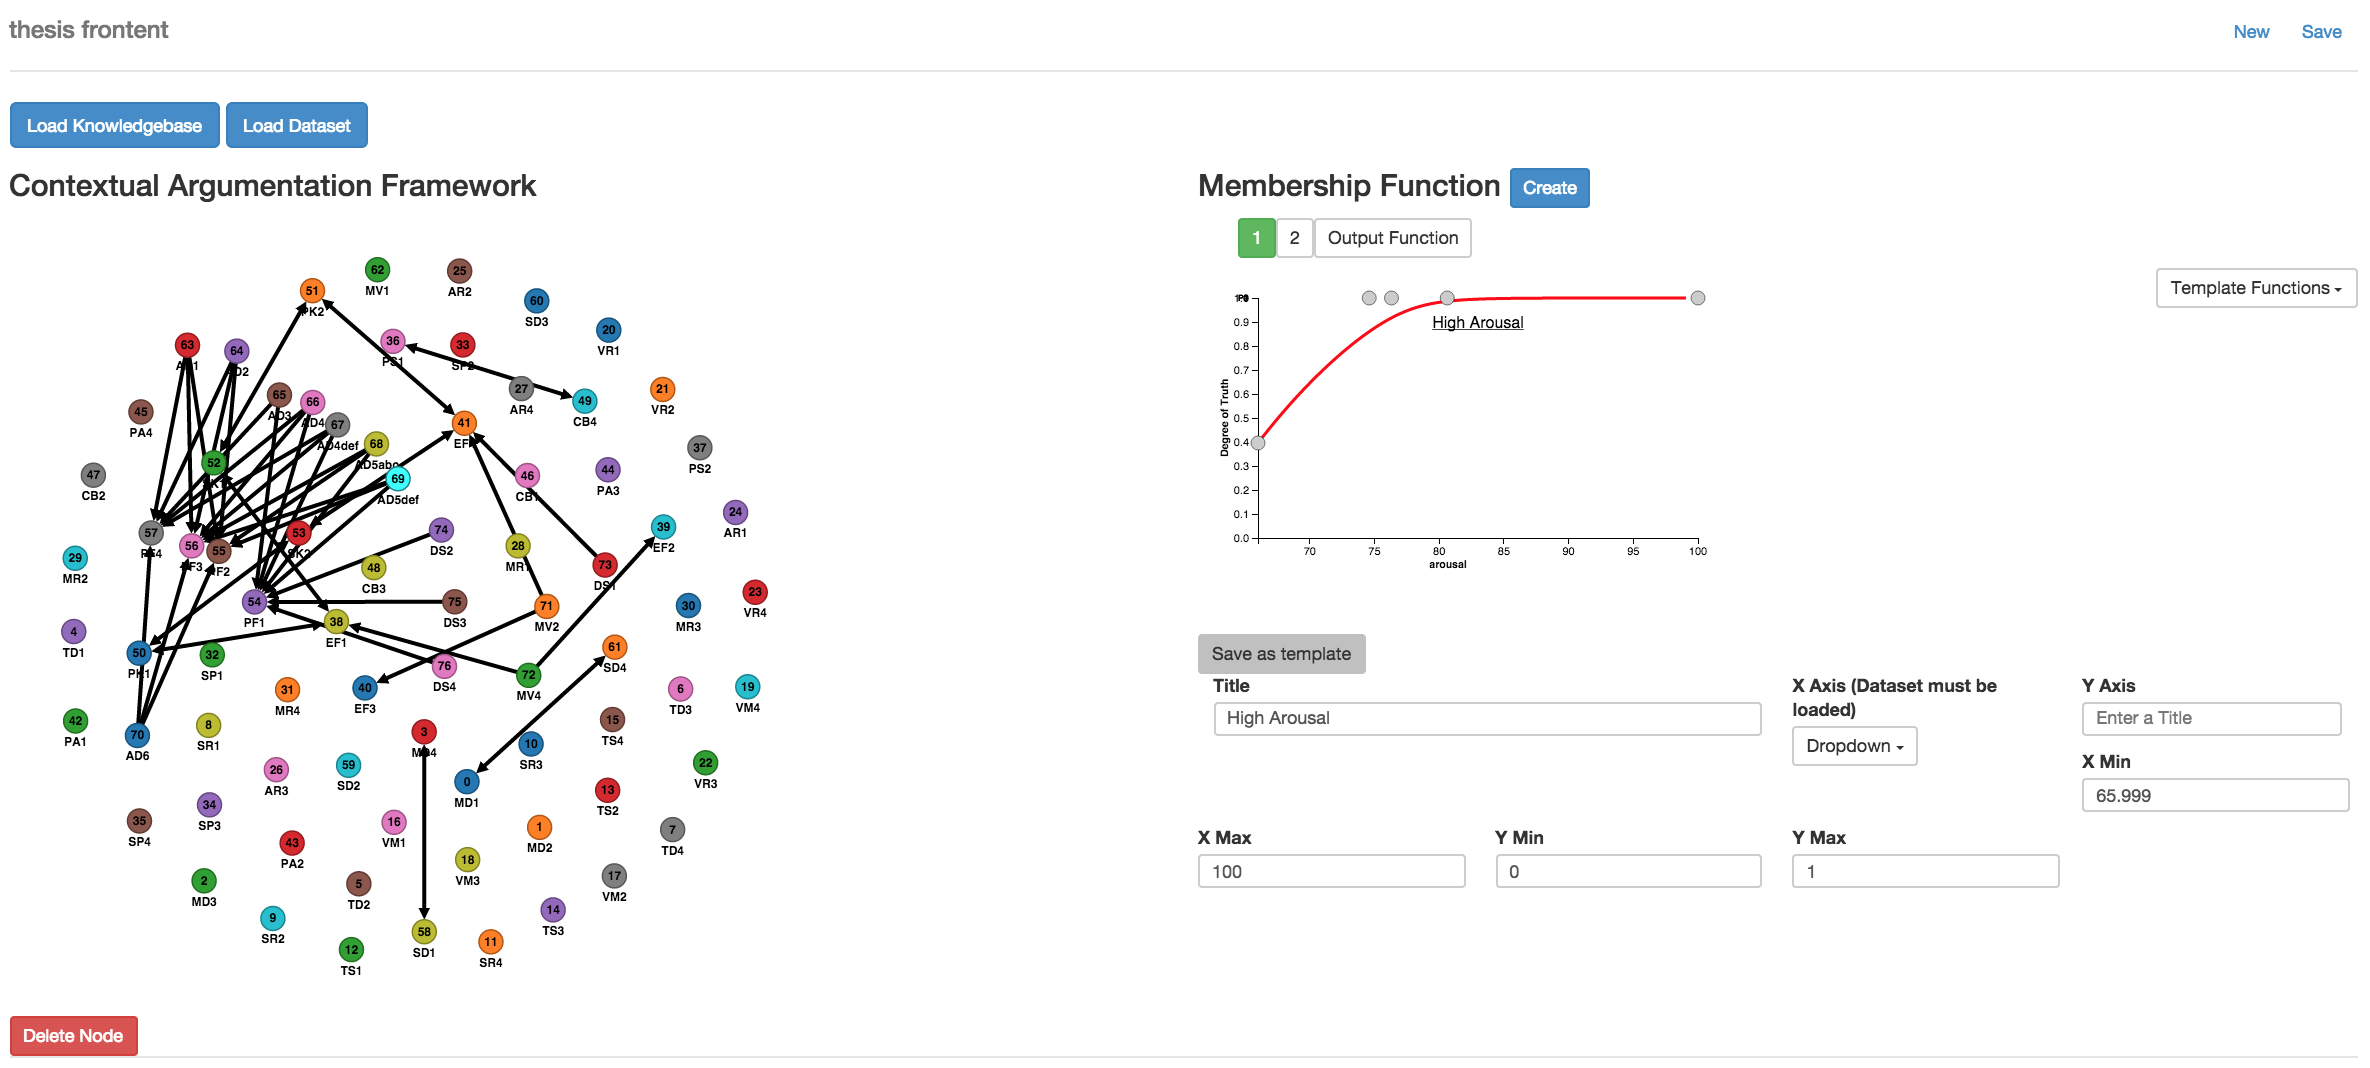
\includegraphics[width=1\textwidth]{Fullscreen}
\caption{The fully developed tool for eliciting knowledge bases}
\end{figure}

\begin{figure}[H]
\centering
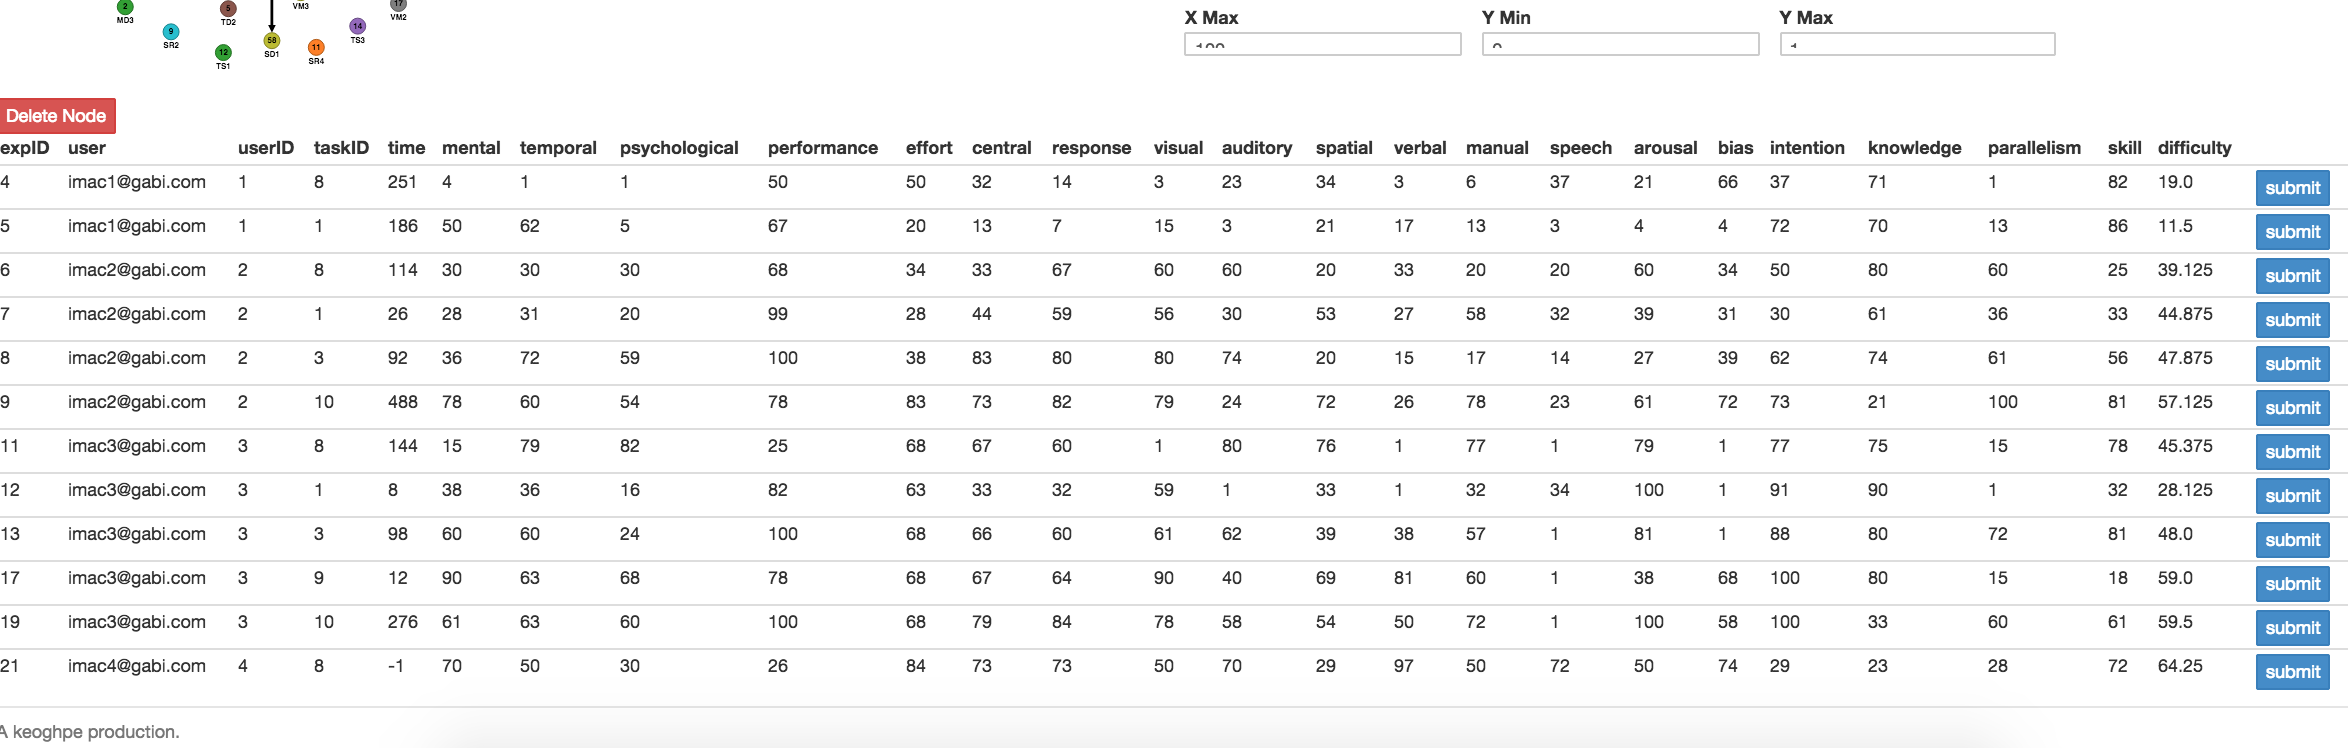
\includegraphics[width=1\textwidth]{data}
\caption{A selection of data for the user to test their knowledge base with}
\end{figure}

\begin{figure}[H]
\centering
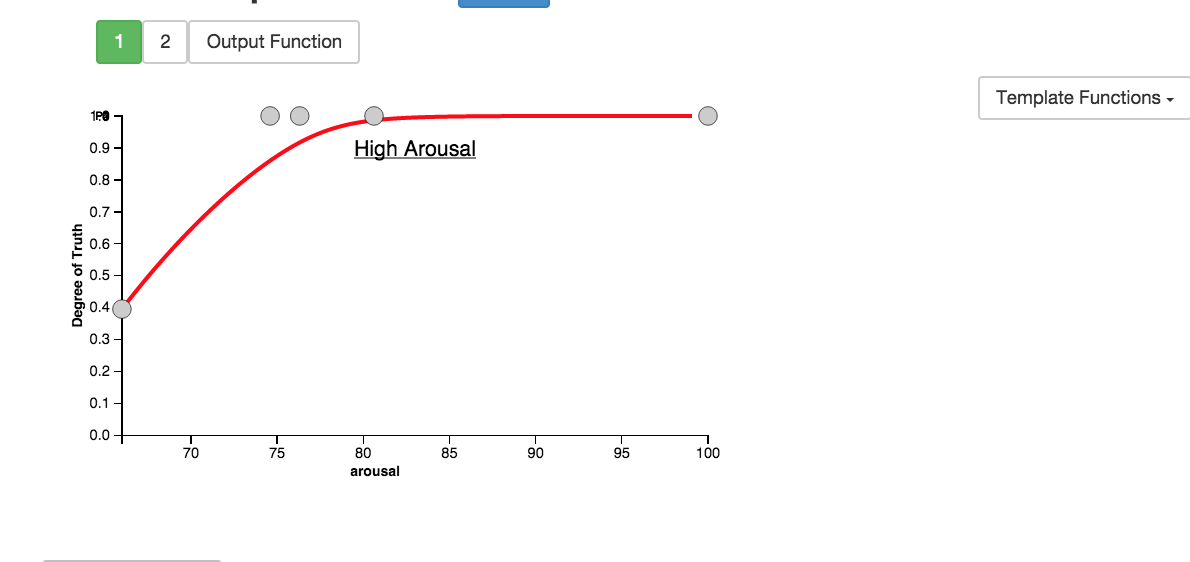
\includegraphics[width=1\textwidth]{membershipfunction}
\caption{An interface that allows a user to `draw' a membership function}
\end{figure}

\begin{figure}[H]
\centering
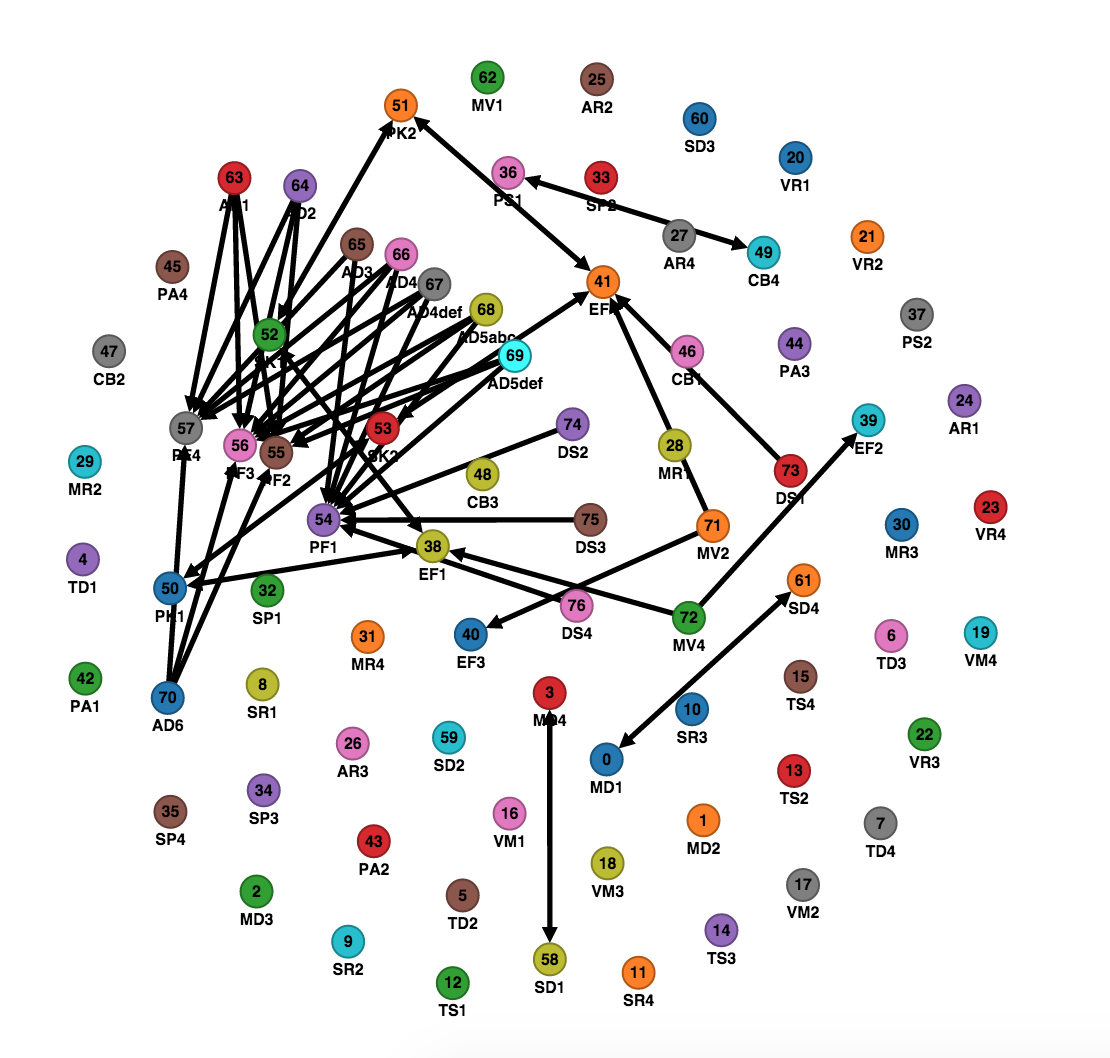
\includegraphics[width=1\textwidth]{ExpertAF}
\caption{The Argumentation Framework developed by the expert using the tool}
\end{figure}

\begin{figure}[H]
\centering
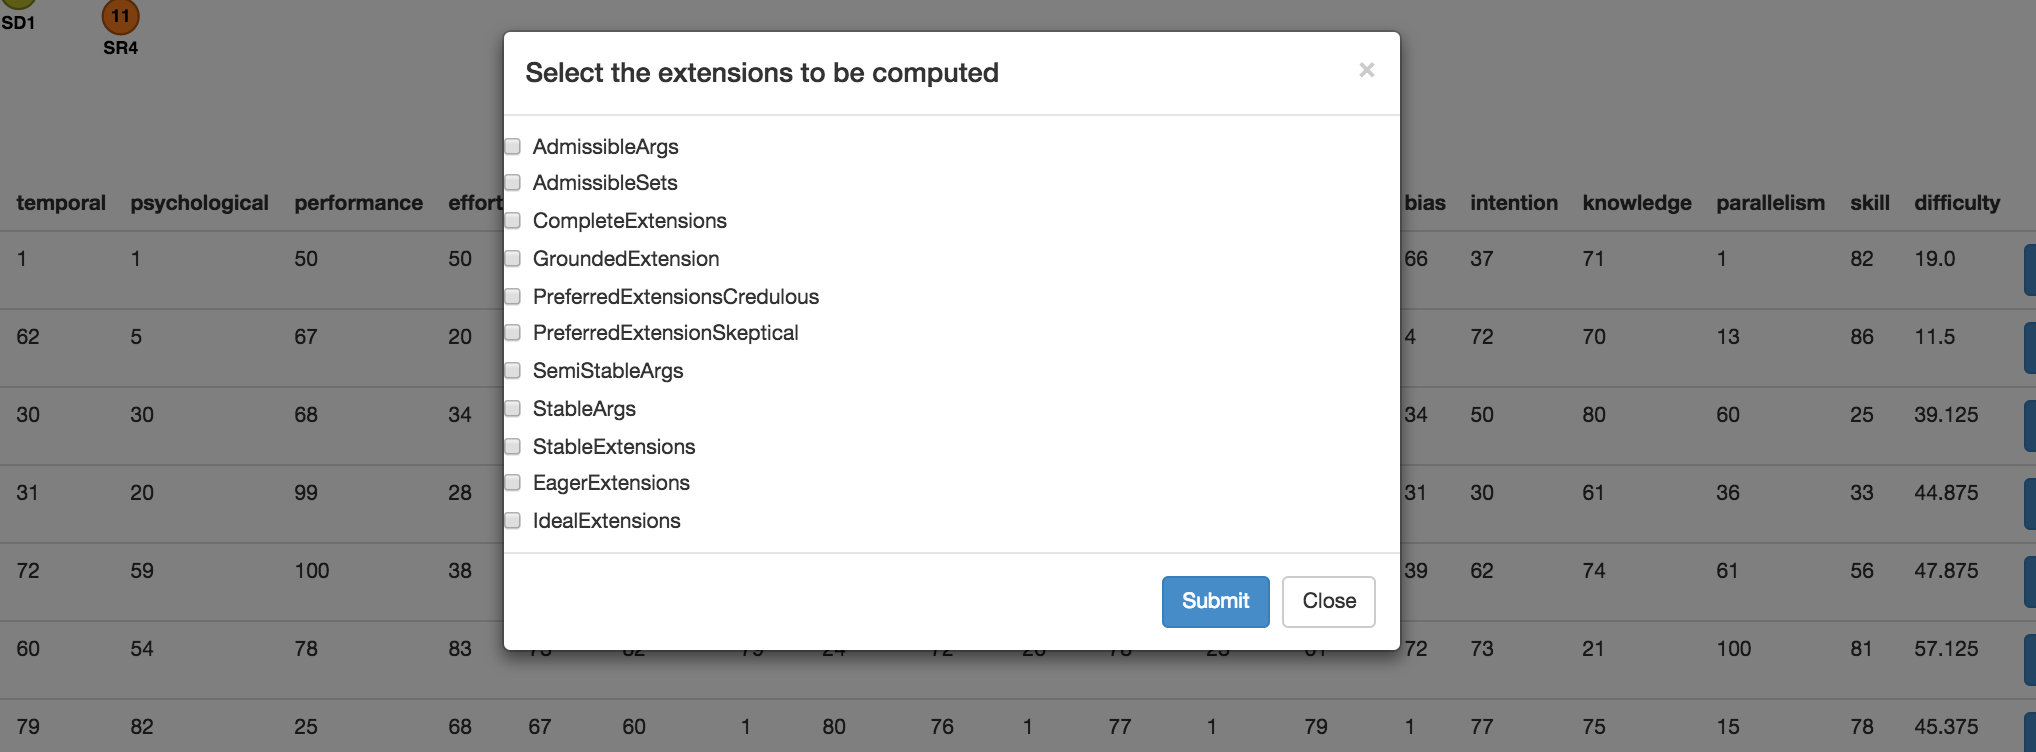
\includegraphics[width=1\textwidth]{options}
\caption{A list of options for semantics that can be computed by the system}
\end{figure}

\begin{figure}[H]
\centering
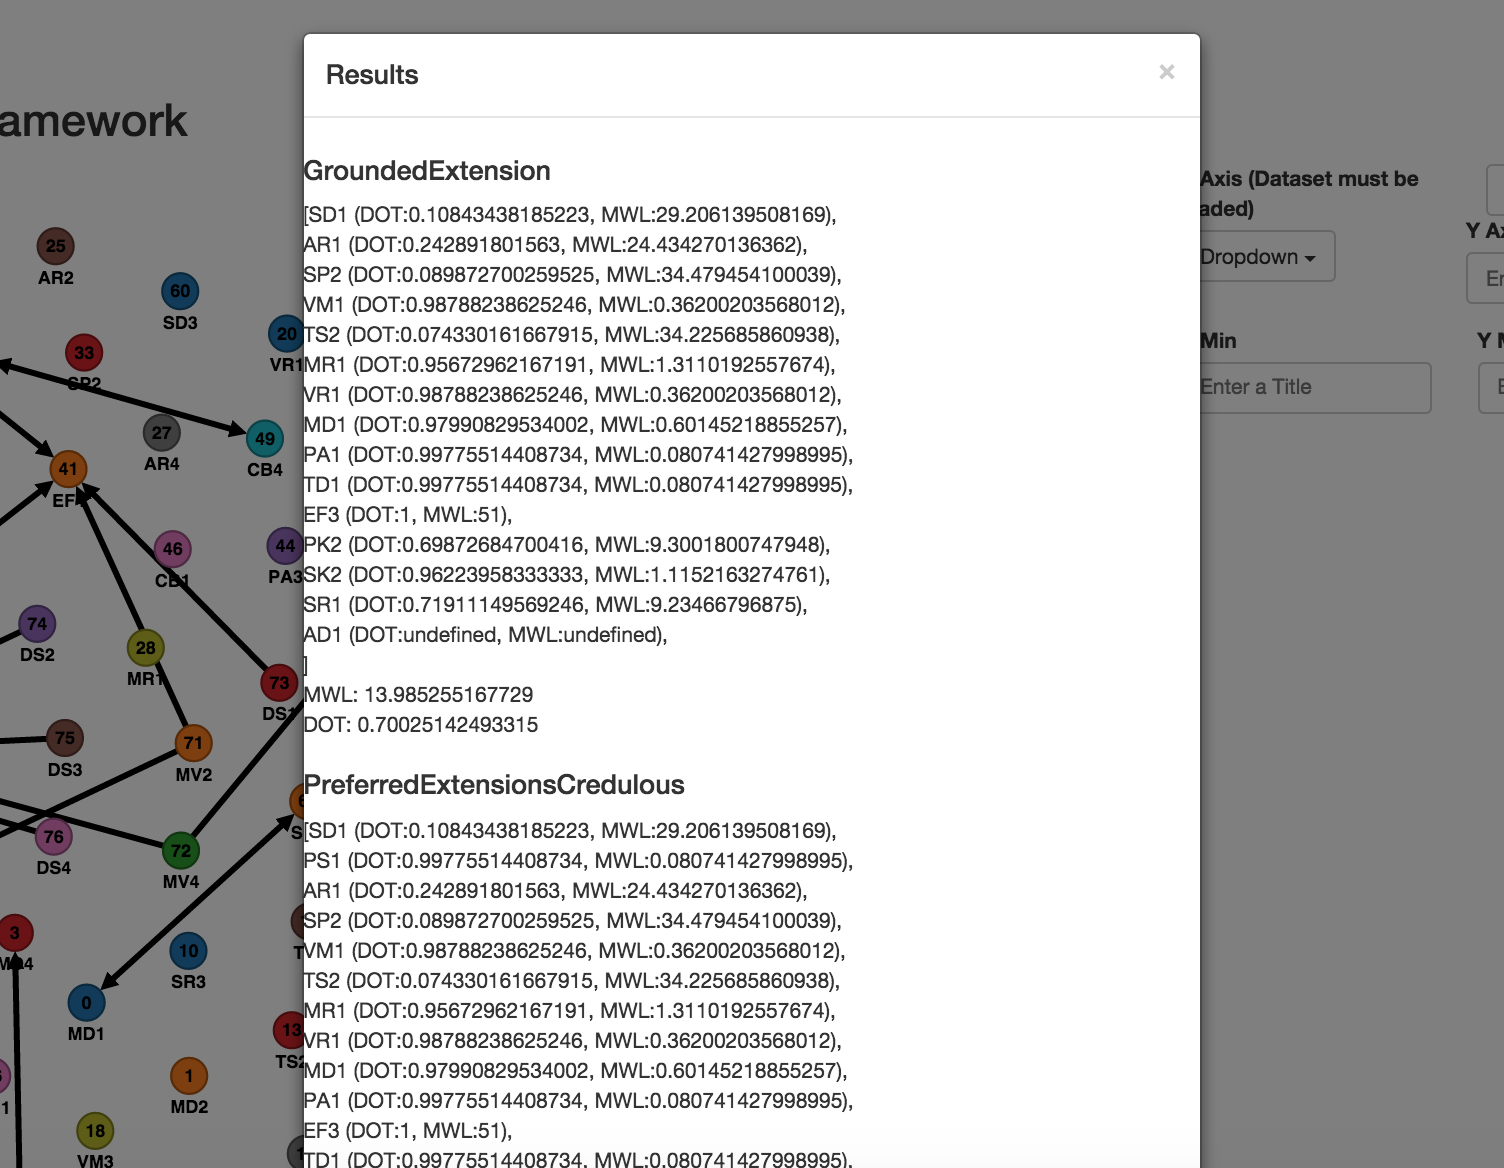
\includegraphics[width=1\textwidth]{results}
\caption{Results of computing the semantics on the framework}
\end{figure}

%----------------------------------------------------------------------------------------
%	SECTION 2
%----------------------------------------------------------------------------------------

\subsection{Generation of Results}



\section{Conclusions}


